\documentclass[10pt,a4paper]{article}
\usepackage[utf8x]{inputenc}
\usepackage{ucs}
\usepackage{amsmath}
\usepackage{amsfonts}
\usepackage{amssymb}
\usepackage{graphicx}
\usepackage{moreverb} 
\usepackage{hyperref}
\usepackage{colortbl}
\pagestyle{headings}

\begin{document}
\renewcommand{\contentsname}{Indice} 
\renewcommand\listfigurename{Lista de Figuras}
\renewcommand\listtablename{Lista de Tablas}
\newcommand\bibname{Bibliografía}
\renewcommand{\refname}{Bibliografía}
\renewcommand\indexname{Indice alfabético}
\renewcommand\figurename{Figura}
\renewcommand\tablename{Tabla}
\renewcommand\partname{Parte}
\newcommand\chaptername{Capítulo}
\renewcommand\appendixname{Apéndice}
\renewcommand\abstractname{Resumen}

\title{Décima semana de trabajo [9 - 13 de Junio]}
\author{Milton Inostroza Aguilera}
\date{16 de Junio de 2008}
\clearpage
\maketitle

\begin{abstract}

Se modifica protocolo de comunicación agregando lo siguiente:
\begin{itemize}
\item \textit{f\_lineno} es agregado a probe
\item \textit{file\_name} es agregado a method/function register
\end{itemize}
\\
Se ha añadido soporte para la correcta registración de las excepciones.  Anteriormente sólo se registraba la primera ocurrencia de una excepción sin examinar si es que esta estaba dentro de un bloque try/except.  El problema anterior se analizó y se implementó la solución que es la de dar soporte para la propagamación de las excepciones.\\

Se ha añadido modificación en tiempo de ejecución de las clases escritas por el programador.  Lo anterior con el objetivo que todas las clases tengan el método \textit{\_\_setattr\_\_} definido de tal forma que el depurador pueda estar notificado de los cambios de valores en los atributos de una determinada instancia. 


\end{abstract}
\newpage
\tableofcontents
\newpage
\listoffigures
\newpage
\listoftables
\newpage
\section{Propagación de excepciones}

El problema que se tenía con el manejo de excepciones era que al momento de encontrar un lanzamiento de excepción registrabamos la salida del método con el tipo de excepción y dejabamos de depurar sin percatarnos si es que esta excepción era lanzada dentro de un bloque try/except, lo cual registraba un comportamiento erroneo de nuestro programa objetivo.\\

Lo que se realizó fue un análisis por los casos bases detectados y estos son los siguientes:

\begin{itemize}
\item Excepción sin try/except en su propio frame y tampoco en sus frames padres
Lo que se realiza en este caso es inspeccionar el bytecode en busca de la instrucción \textit{SETUP\_EXCEPT}, si es que esta instrucción no está presente dentro del bloque correspondiente, se marca el retorno del método / función con la excepción correspondiente y el atributo \textit{self.FLAG\_THROWN} es marcado con el valor \textit{True}.  Con esto dejamos libre el flujo normal del programa a la espera de los siguientes eventos que sucedan en el programa objetivo.

\item Excepción sin try/except en su propio frame pero si en algún frame padre
En el punto anterior al dejar seguir el flujo normal del programa la excepción y si no es capturada en el mismo frame pero si en un frame superior, el depurador lo que hace es inspeccionar el bytecode en busca de la instrucción anteriormente señalada y si la encuentra el depurador es inhibido de hacer cualquier acción, ya que todos los retornos que haya producido la excepción ya han sido registrados correctamente.

\end{itemize}
\newpage

\section{Modificación de clases en tiempo de ejecución}

En informes anteriores se ha descrito la utilidad de la clase interna llamada Descriptor.  Hasta el momento para realizar las pruebas de depuración, todas las clases escritas debían heredar de la clase Descriptor para que el depurador pudiera realizar el trabajo de inspeccionar los cambios de los atributos de cada clase.  Obligar a un programador a escribir la herencia es bastante incomodo ya que es bastante antinatural tener que modificar parte de su código para que este sea depurado y luego volver a cambiarlo, quitando notablemente usabilidad al depurador propuesto.\\

Se trabajó por varias direcciones: a) Modificar el atributo \textit{\_\_bases\_\_}, b) Modificar el bytecode, c) Modificar en tiempo de ejecución el diccionario \textit{\_\_dict\_\_} de la clase definida por el programador.  Después de una semana de estudio las opciones a) y b) fueron deshechadas y la opción c) fue la elegida para implementar.\\

Básicamente lo que se realiza es que al momento que el programador termina de definir su clase el depurador toma esta definición y modifica el diccionario local de la clases agregando un atributo más y este es el atributo \textit{\_\_setattr\_\_} definido en la clase Descriptor.  Si bien es cierto que la clase Descriptor ya no será usada directamente por el programador si será utilizada directamente por el depurador.  Es por esta razón que no será eliminada del depurador.


\newpage
\section{Depuraciones}

Después de haber solucionado los problemas anteriormentes descritos, ya podemos ver la intefaz gráfica funcionando de forma más completa.\\

Se ha depurado experimentalmente el siguiente trozo de código:\\

\begin{verbatim}
    
class clase1(object):
    
    def __init__(self, y):
        self.x = 1
        self.c = 2
        self.z = 1
        self.metodo(self.z, 1, 2, 3)
        return
    
    def metodo(self, h, i, j, k):
        self.casa = 1 + h
        h = 0
        print self.z
        k = i + j
        self.x = k
        self.foo()
        return k
    
    def foo(self):
        y = 1/0
\end{verbatim}

TOD, nos muestra la siguiente información:\\

\begin{figure}[hpb]
	\centering
	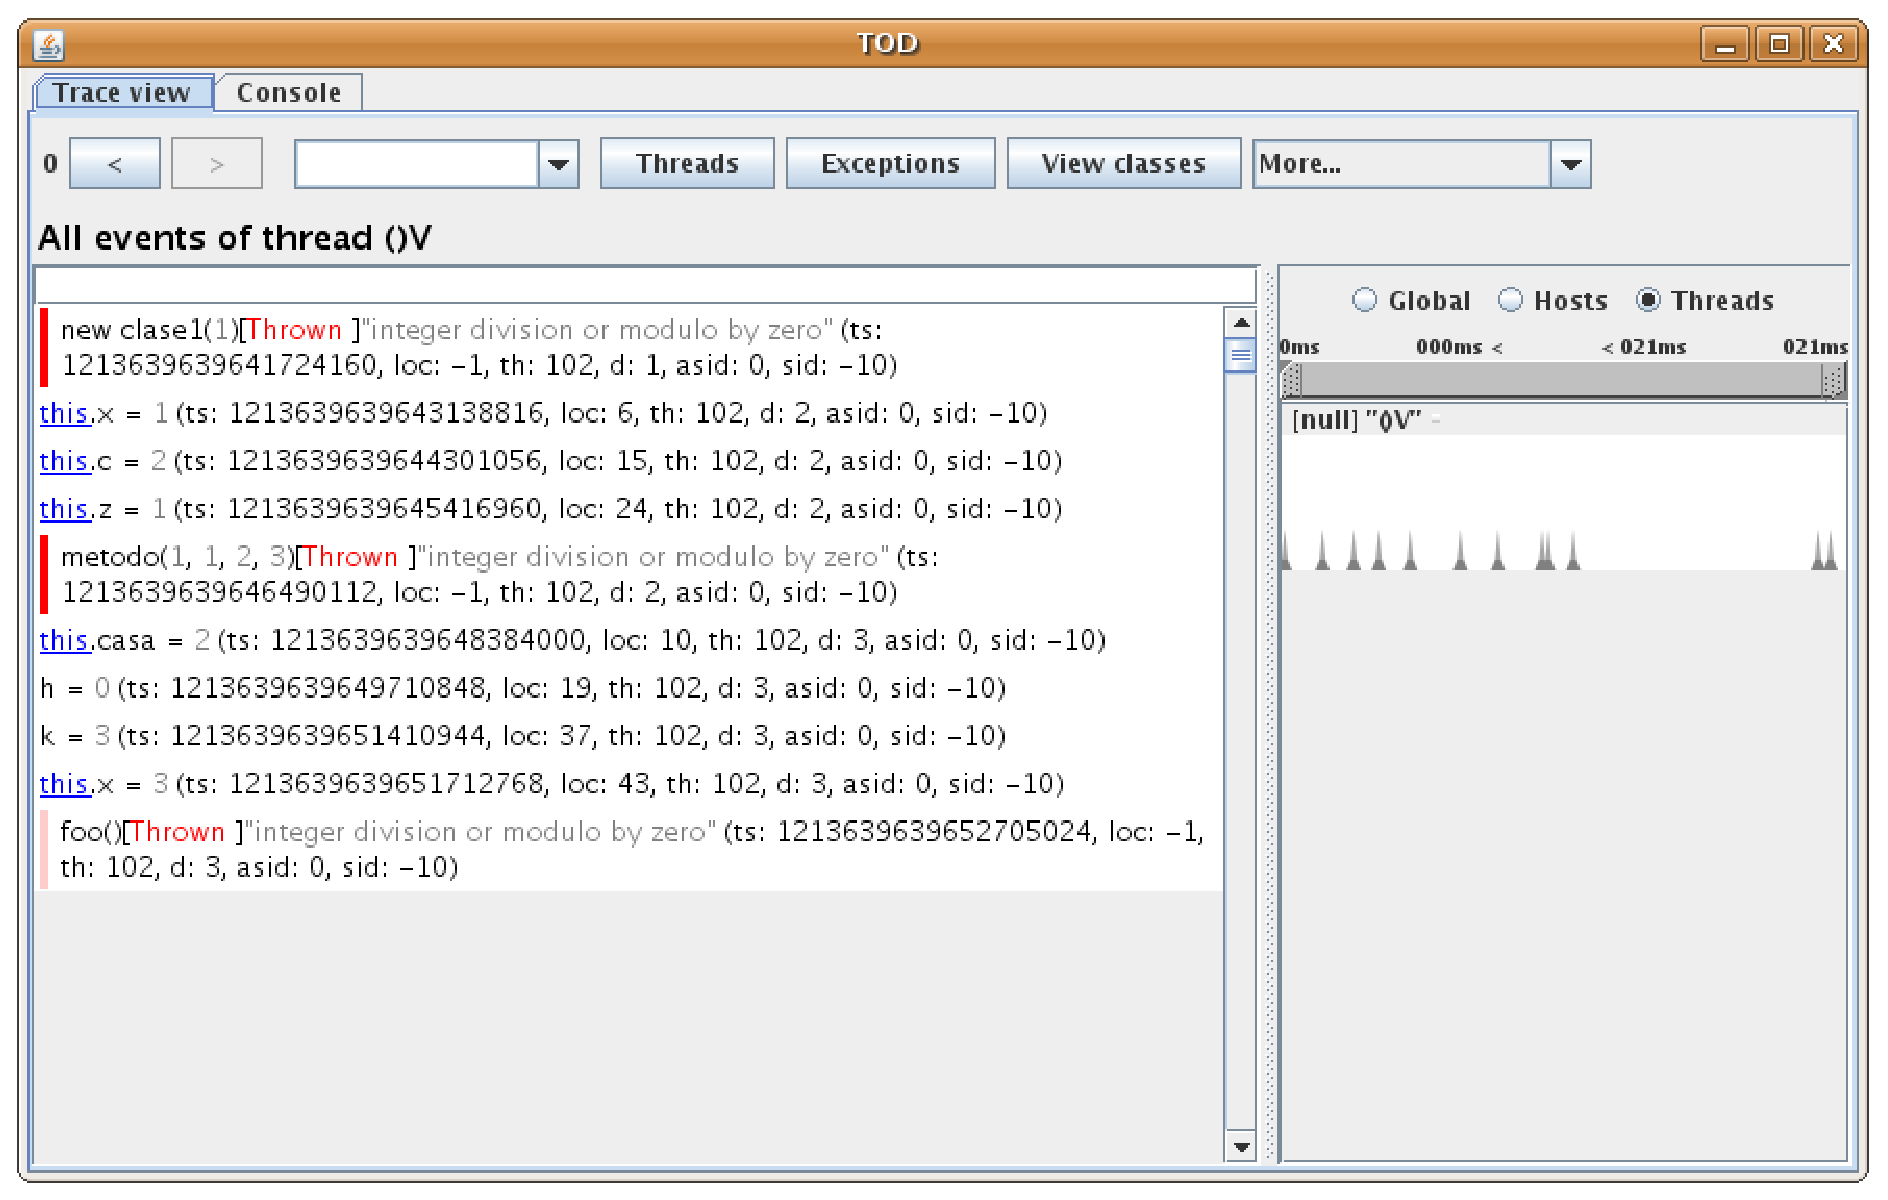
\includegraphics[scale=0.3]{images/TOD-1.eps}
	\caption{script depurado, caso 1}
\end{figure}

Se ha depurado experimentalmente el siguiente trozo de código:\\

\begin{verbatim}
    
class clase1(object):
    
    def __init__(self, y):
        self.x = 1
        self.c = 2
        self.z = 1
        self.metodo(self.z, 1, 2, 3)
        return
    
    def metodo(self, h, i, j, k):
        self.casa = 1 + h
        h = 0
        print self.z
        k = i + j
        self.x = k
        try:
            o = self.foo()
        except:
            o = 1
        return k
    
    def foo(self):
        y = 1/0
\end{verbatim}


TOD, nos muestra la siguiente información:\\
\newpage
\begin{figure}[hpb]
	\centering
	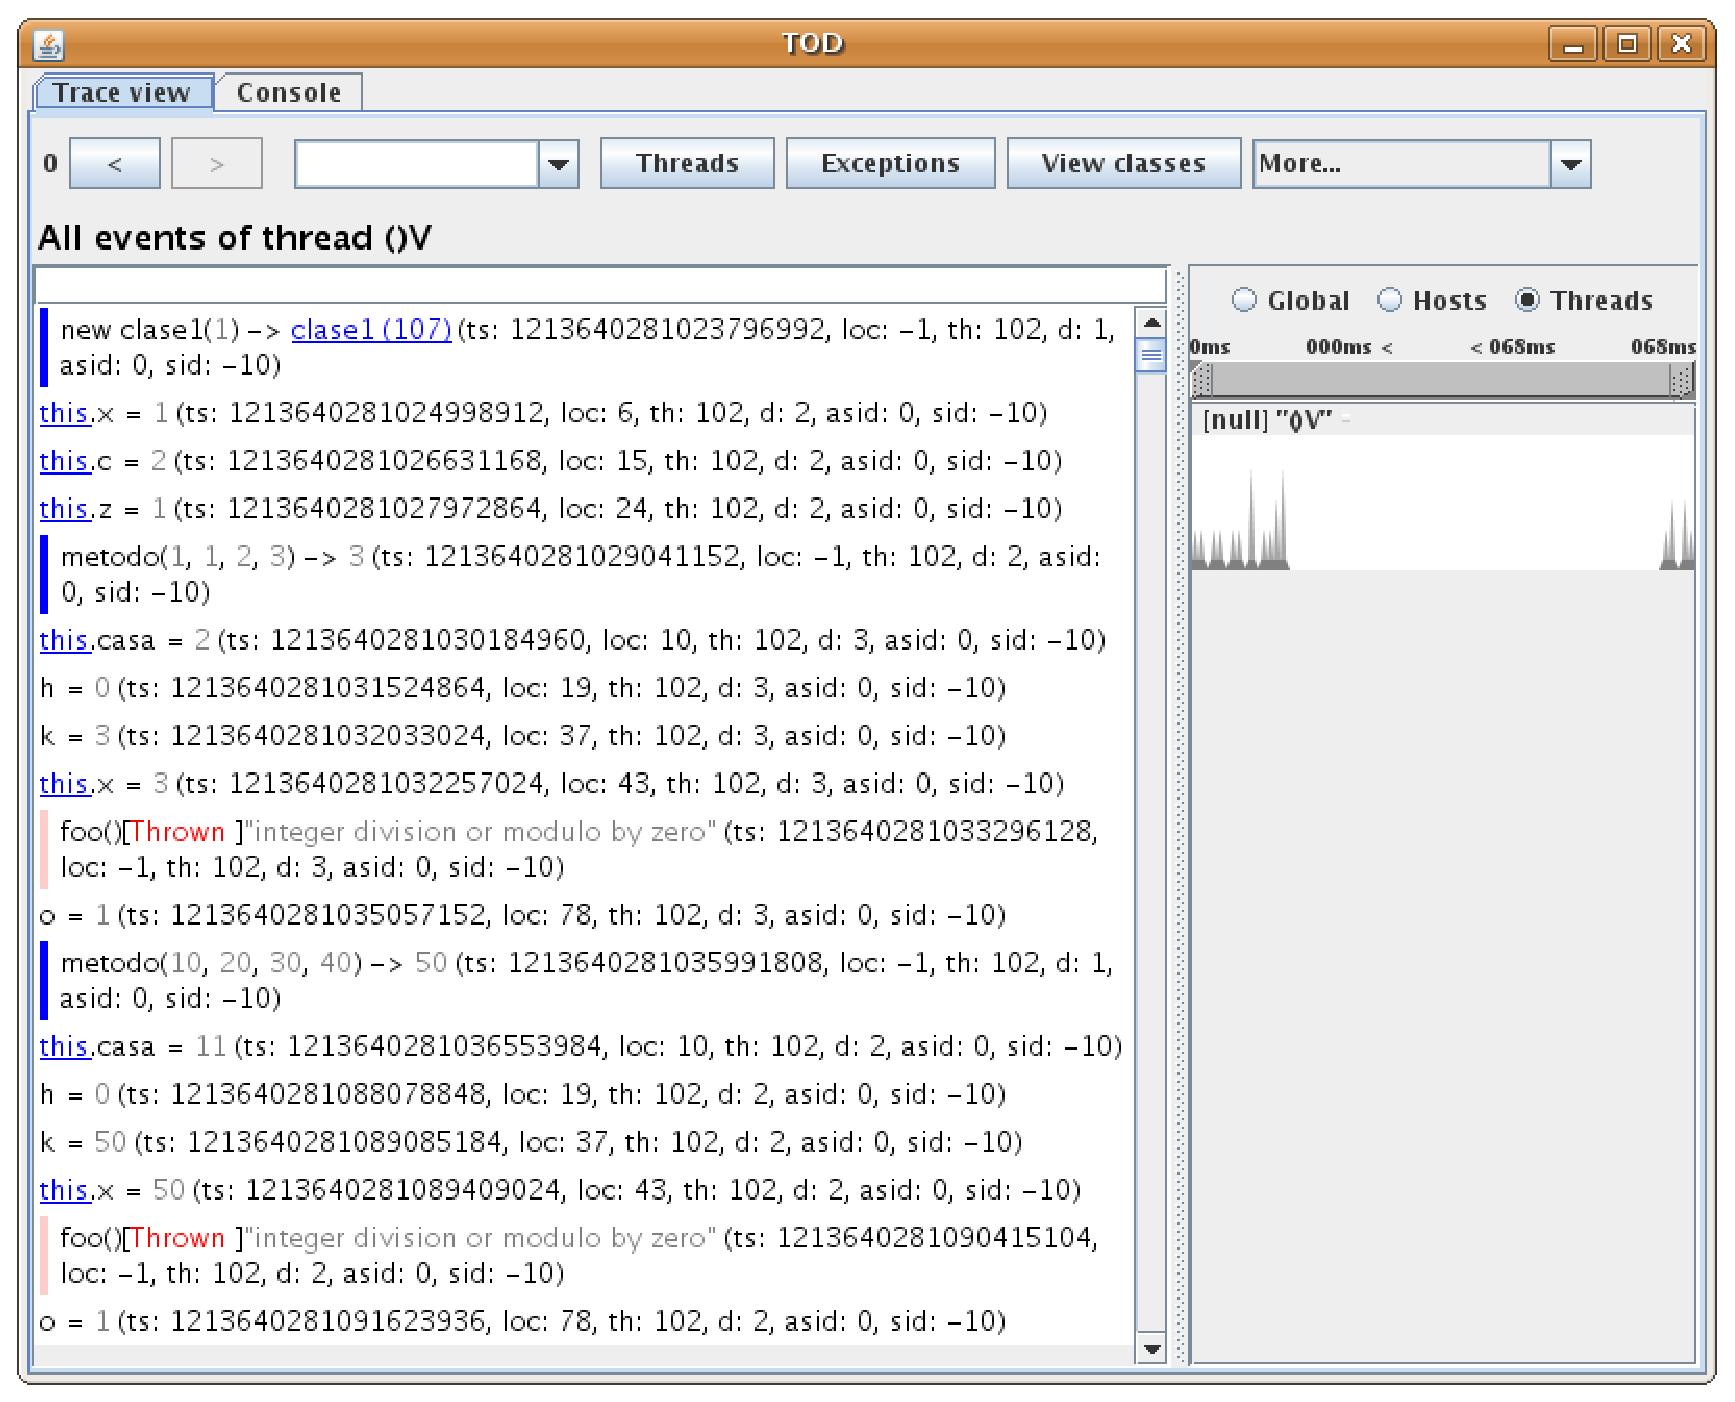
\includegraphics[scale=0.3]{images/TOD-2.eps}
	\caption{Vista de todos los eventos}
\end{figure}

Es importante señalar que en los casos anteriores se muestra el correcto funcionamiento de la propagación de las excepciones y la no utilización por parte del programador de la herencia a la clase Descriptor.

\newpage
\begin{thebibliography}{2}
\bibitem{bytecode} \url{http://docs.python.org/lib/bytecodes.html}
\end{thebibliography}
\end{document}
